\pretocmd{\chapter}{\glsresetall}{}{}

\chapter{Results}

\label{Results}

This chapter presents the main outcomes of the proposed\ac{mcts}-based approach for\ac{cb-ctt}. The following sections explore aspects such as computational performance, feasibility of generated timetables, analysis of the exploration constant \(C\), the impact of pruning, effectiveness of the diving strategy, and a comparison against benchmark competition results.

\section{Python vs PyPy Performance}

During the development and testing of the method, both standard Python and PyPy\footnote{A Just-In-Time (JIT) python compiling alternative. Link: \url{https://pypy.org/}} were evaluated for performance. While both correctly executed the\ac{mcts} algorithm, the performance difference was substantial. PyPy called over three times more functions compared to Python.

Given the compute-intensive nature of\ac{mcts}, PyPy was ultimately chosen for running all the experiments and benchmarks.

\section{Feasibility}

One of the fundamental requirements of\ac{cb-ctt} is the ability to produce feasible schedules, i.e., timetables that strictly adhere to hard constraints such as avoiding room clashes, overlapping events, and unavailable periods.

Throughout all experiments, the proposed method consistently produced feasible solutions across all tested datasets from the\ac{itc-2007} benchmark. This demonstrates the robustness of the method's constraint handling mechanisms, regardless of instance size or structural complexity, confirming the general applicability of the approach.

\section{Random Simulation Performance}

To establish a baseline for the effectiveness of guided search, a random simulation test was conducted.  In this configuration, event, period, and room assignments were selected at random, without considering constraint satisfaction or search tree statistics. The goal of this experiment was to evaluate the ability of a purely stochastic method to find feasible solutions and to compare its performance against the guided\ac{mcts} approach. 

Across multiple runs, the random simulation consistently failed to produce feasible solutions. Although random simulations can execute a high number of iterations due to its simplicity and lack of tree maintenance overhead, the majority of these iterations were ineffective, repeatedly exploring infeasible parts of the search space. 

These results highlight the importance of incorporating domain knowledge information to ensure feasibility in a realistic time frame.

\section{\(C\) Parameter Behaviour}

The exploration constant \(C\) in the\ac{uct} formula (Formula \ref{uct_formula}) was varied across several orders of magnitude (from 0.1 to 1000), including the modified variant incorporating accumulated rewards (Equation \ref{modified_uct}). 

Surprisingly, the results showed that varying \(C\) had minimal impact on solution quality, which indicates a lower-than-expected sensitivity to node selection.

\section{Pruning}

The application of pruning during\ac{mcts} plays a crucial role in the efficiency of the search process.

Figure \ref{fig:without_pruning_result} illustrates the behavior of the method without pruning. The search frequently explores infeasible branches of the tree, which is evident from the large number of iterations with hard constraint violations. Although some feasible solutions are eventually discovered, the overall search efficiency is compromised due to the continuous evaluation of solutions that will be ultimately discarded.

Conversely, when pruning is applied (Figure \ref{fig:pruning_result}), the search is restricted to branches that satisfy hard constraints. As a result, the hard constraint value remains consistently at zero throughout the iterations, reflecting that pruning effectively excludes infeasible regions from the search space. This restriction allows\ac{mcts} to focus on high-quality and valid solutions, preventing wasteful exploration. The cleaner progression and stable constraint satisfaction not only accelerate convergence but also improve the overall robustness of the approach. 

While not depicted in Figure \ref{fig:pruning_result}, it is worth noting that simulations may still experience occasional hard constraint violations because pruning is applied to branches within the tree rather than across the entire search space.

\begin{figure}
 \centering
     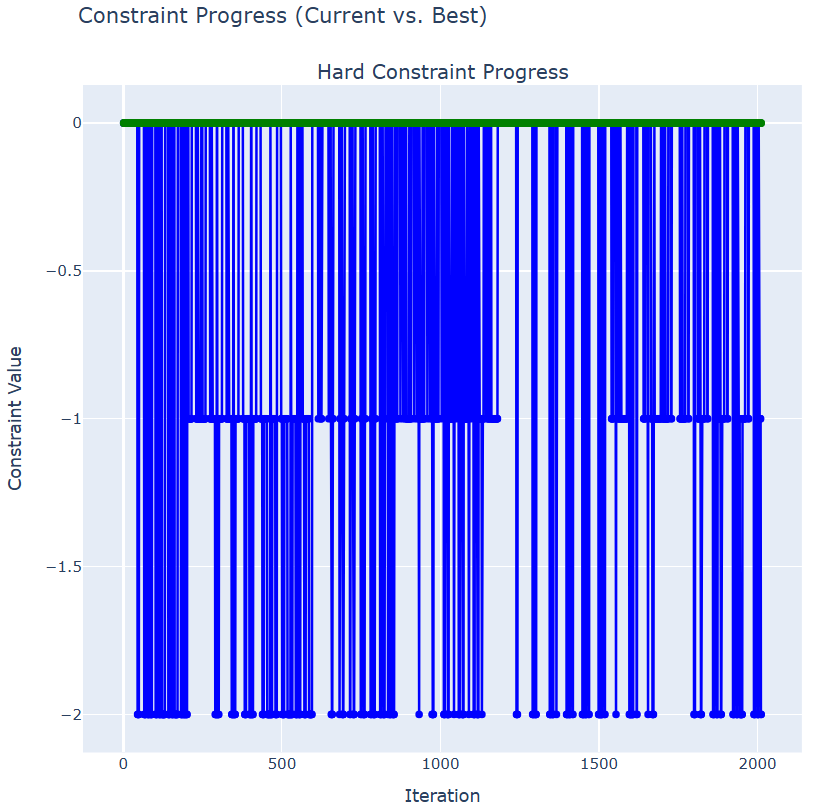
\includegraphics[width=0.6\columnwidth]{Results/without_pruning.png}
     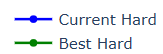
\includegraphics[width=0.2\columnwidth]{Results/hard_caption.png}
     \caption{Hard constraint progress without pruning during 10 minutes on the \texttt{comp01} instance from\ac{itc-2007}.}
     \label{fig:without_pruning_result}
\end{figure}

\begin{figure}
 \centering
    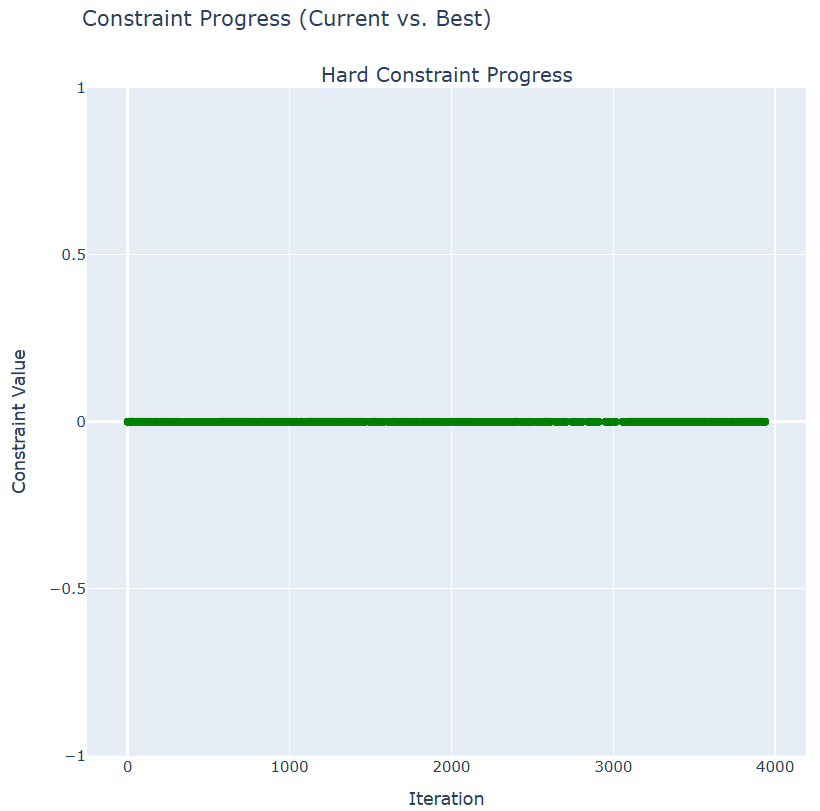
\includegraphics[width=0.6\columnwidth]{Results/pruning.png}
    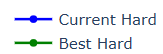
\includegraphics[width=0.2\columnwidth]{Results/hard_caption.png}
    \caption{Hard constraint progress with pruning during 10 minutes on the \texttt{comp01} instance from\ac{itc-2007}.}
    \label{fig:pruning_result}
\end{figure}

\section{Hill Climbing}

To improve solution quality,\ac{hc} was combined with the\ac{mcts} algorithm (chapter \ref{Development} section \ref{hill_climbing_section}). Importantly,\ac{hc} operates exclusively on complete feasible solutions returned by\ac{mcts}, ensuring that hard constraint validity is maintained throughout the optimization process.

However, the integration of\ac{hc} did not consistently yield lower soft constraint penalties across all tested instances within the 10-minute time limit (Table \ref{tab:comparison_results}). In some cases, the baseline\ac{mcts} approach and the version with the diving strategy achieved comparable or even superior results. This outcome suggests that the effectiveness of local refinement may depend on the quality of the improved solutions generated by \ac{hc}, as well as the number of idle iterations, which is an aspect that, unfortunately, was not properly explored.

Despite the results and the additional computational overhead introduced by\ac{hc}, it still demonstrates potential to provide meaningful improvements in solution quality.
   
\section{Diving}

To improve the convergence speed and solution quality during timetable generation, the\ac{mcts} algorithm incorporates a diving strategy (chapter \ref{Development} section \ref{sec:diving}). Moreover, the diving strategy complements pruning by directing attention to already feasible branches. This method helps concentrate computational resources on areas of the search space that are both valid and high quality.

Figures \ref{fig:diving_result} and \ref{fig:without_diving_result} show the soft constraint penalty progression over time on the \texttt{comp01} instance from the\ac{itc-2007} benchmark, using and not using the diving strategy.

The results demonstrate that the diving mechanism contributes positively to the search effectiveness:

\begin{itemize}
\item \textbf{Faster convergence:} The algorithm reaches lower penalty regions more rapidly compared to a standard breadth-oriented\ac{mcts} approach. By tracking and expanding the most promising nodes first, the diving queue helps avoid wasting iterations on less promising parts of the tree.

\item \textbf{Improved solution quality:} As observed in the soft penalty trend, the use of diving leads to an improvement compared to the approach without diving (Figure \ref{fig:without_diving_result}). This improvement is only noticeable when we extend the run time. This shows that the diving strategy not only accelerates convergence but also contributes to reaching higher-quality solutions.

\item \textbf{Focused exploitation:} The queue-based selection mechanism ensures that the algorithm deepens the most promising paths. In practice, this limits unnecessary expansion of under-performing nodes and encourages building upon solutions with known potential.
\end{itemize}

\begin{figure}
 \centering
    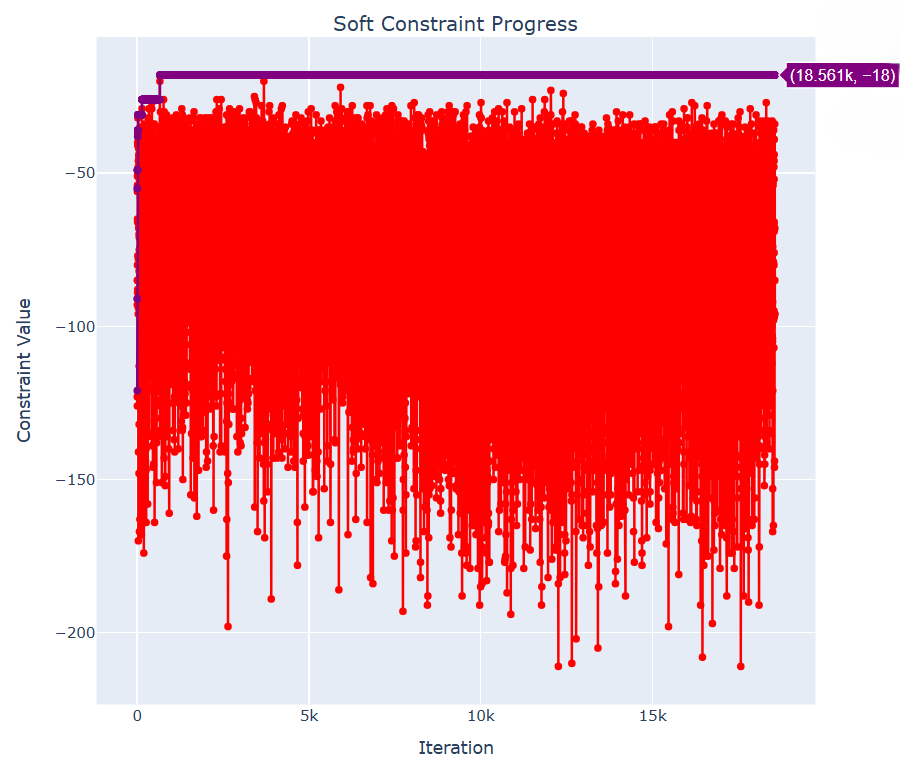
\includegraphics[width=0.8\columnwidth]{Results/without_diving_result.png}
    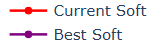
\includegraphics[width=0.19\columnwidth]{Results/soft_caption.png}
    \caption{Soft constraint progress without using the diving approach on the \texttt{comp01} instance from\ac{itc-2007} for 1 hour and \(C\)=1.4.}
    \label{fig:without_diving_result}
\end{figure}

\begin{figure}
 \centering
    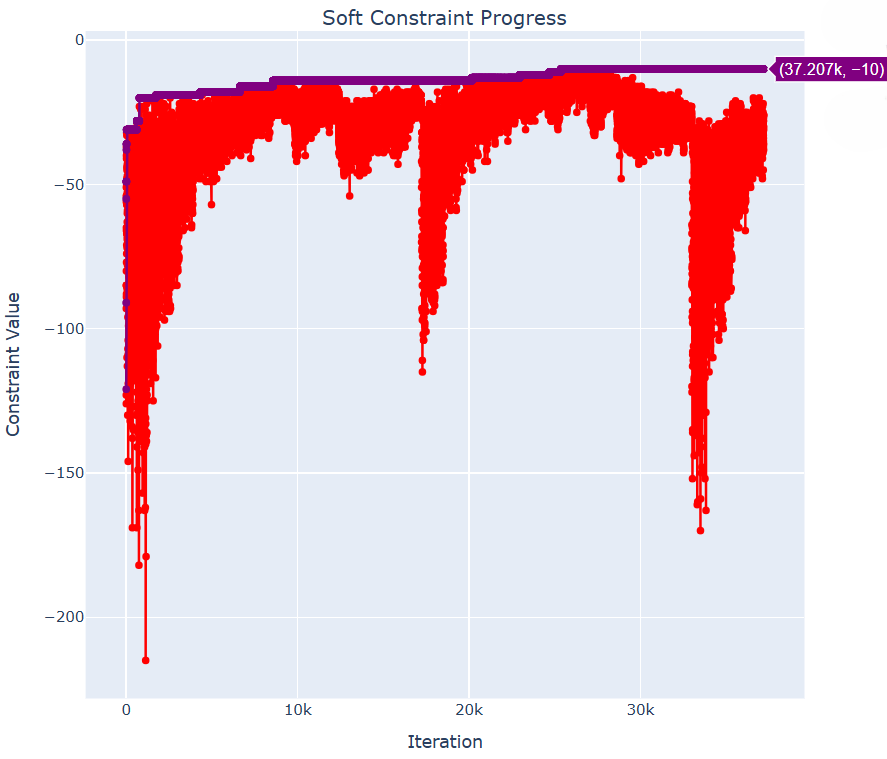
\includegraphics[width=0.8\columnwidth]{Results/diving_result.png}
    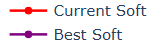
\includegraphics[width=0.19\columnwidth]{Results/soft_caption.png}
    \caption{Soft constraint progress using the diving approach on the \texttt{comp01} instance from\ac{itc-2007} for 1 hour and \(C\)=1.4.}
    \label{fig:diving_result}
\end{figure}

In both approaches (with and without diving) it is noticeable that the algorithm eventually stagnates, reaching a point where no further improvement is observed. After an initial phase of rapid improvement, the soft penalty score typically plateaus without finding an optimal solution. However, with the diving strategy, the soft constraint penalties at each iteration tend to remain closer to the best solution found, indicating a more stable and focused search trajectory.

\section{Competition Results Comparison}

The effectiveness of the\ac{mcts}-\ac{hc} hybrid was evaluated on the official\ac{itc-2007} track 3 benchmark datasets. Table \ref{tab:comparison_results} presents a comparison between the best results submitted by Müller (competition winner) and our approach (with \(C\)=0.1) for instances \texttt{comp01.ctt} to\texttt{comp05.ctt}, and \texttt{comp11.ctt}. Initially, all benchmark instances were considered for evaluation, but due to time constraints, the experiments were narrowed down to focus on only six instances.

\begin{sidewaystable}[p]
\centering
%\footnotesize
\setlength{\tabcolsep}{3pt}
\begin{tabular}{lccc|ccc|ccc|ccc|ccc}
\hline
\textbf{Instance}
& \multicolumn{3}{c|}{\textbf{Müller}} 
& \multicolumn{3}{c|}{\textbf{Random Simulation}} 
& \multicolumn{3}{c|}{\textbf{\ac{mcts}+\ac{hc}}} 
& \multicolumn{3}{c|}{\textbf{\ac{mcts}+Diving}} 
& \multicolumn{3}{c}{\textbf{\ac{mcts}+\ac{hc}+Diving}} \\
& avg & max & min 
& avg & max & min 
& avg & max & min 
& avg & max & min 
& avg & max & min \\
\hline
\textbf{comp01} & 5 (0) & 5 (0) & 5 (0) & 2136.8 (96.1) & 2469 (99) & 1844 (91) & (0) & (0) & (0) & 18 (0) & 22 (0) & 12 (0) & 17.4 (0) & 23 (0) & 12 (0) \\
\textbf{comp02} & 61.3 (0) & 70 (0) & 51 (0) & 8099.1 (231.9) & 9351 (236) & 6909 (228) & (0) & (0) & (0) & 213.1 (0) & 227 (0) & 190 (0) & 208.2 (0) & 232 (0) & 186 (0) \\
\textbf{comp03} & 94.8 (0) & 103 (0) & 84 (0) & 5941.1 (184.5) & 6575 (187) & 5299 (182) & (0) & (0) & (0) & 251 (0) & 262 (0) & 243 (0) & 241.6 (0) & 260 (0) & 215 (0) \\
\textbf{comp04} & 42.8 (0) & 48 (0) & 37 (0) & 5168.2 (179.8) & 5552 (183) & 4407 (176) & (0) & (0) & (0) & 149.2 (0) & 159 (0) & 142 (0) & 140.9 (0) & 151 (0) & 127 (0) \\
\textbf{comp05} & 343.5 (0) & 379 (0) & 330 (0) & 8752.1 (121.6) & 9482 (125) & 7922 (118) & (0) & (0) & (0) & 633.3 (0) & 700 (0) & 546 (0) & 639.6 (0) & 766 (0) & 587 (0) \\
\textbf{comp11} & 0 (0) & 0 (0) & 0 (0) & 2033.8 (68.8) & 2211 (72) & 1826 (64) & (0) & (0) & (0) & 12.6 (0) & 14 (0) & 11 (0) & 9.9 (0) & 13 (0) & 7 (0) \\
\hline
\end{tabular}
\caption{Comparison of Müller and our method variants across six benchmark instances during 10 minutes. Soft constraint penalties are shown with hard constraint violations in parentheses.}
\label{tab:comparison_results}
\end{sidewaystable}


Although our approach does not yet outperform state-of-the-art methods in terms of soft constraint minimization, even with an extended time, it consistently finds feasible solutions within reasonable time limits. This confirms its robustness and potential as a foundation for further refinement.

\section{Summary}

This chapter evaluated the\ac{mcts}-\ac{hc} hybrid approach across several dimensions: implementation performance, feasibility, parameter tuning, pruning impact, and solution quality. Key findings include:

\begin{itemize}
\item \textbf{Feasibility:} The method consistently generated feasible timetables in the challenging\ac{itc-2007} set of benchmark instances.

\item \textbf{Performance:} PyPy significantly outperformed standard Python, justifying its use in all experiments.

\item \textbf{Random Simulation:} Purely random simulations failed to produce feasible solutions, emphasizing the necessity of guided search and domain knowledge to navigate the complex solution space effectively.

\item \textbf{Pruning:} Efficiently eliminated some infeasible branches, improving search focus and convergence.

\item \textbf{Diving:} Diving successfully reduced soft constraint penalties after\ac{mcts} found a feasible solution.

\item \textbf{Competition Benchmarking:} Although solution quality was below the best-known results, the approach shows solid potential with room for improvement.
\end{itemize}